\documentclass[conference]{IEEEtran}
\IEEEoverridecommandlockouts

\usepackage{cite}
\usepackage[portuguese,brazil]{babel}
\usepackage{amsmath, amssymb, amsfonts}
\usepackage[utf8]{inputenc}
\usepackage{algorithmic}
\usepackage{graphicx}
\usepackage{textcomp}
\usepackage{subfig}
\usepackage{diagbox}
\def\BibTeX{{\rm B\kern-.05em{\sc i\kern-.025em b}\kern-.08em
    T\kern-.1667em\lower.7ex\hbox{E}\kern-.125emX}}
\begin{document}

\title{MO444 - Machine Learning - Relatório da Atividade \#1}

\author{\IEEEauthorblockN{Bárbara Caroline Benato}
\IEEEauthorblockA{
RA 192865\\
barbarabenato@gmail.com}
\and
\IEEEauthorblockN{Breno Leite}
\IEEEauthorblockA{
RA 192863\\
brenolleite@gmail.com}}

\maketitle

\section{Introdução}

A primeira atividade da disciplina de \textit{Machine Learning} (MO444) tem como intuito explorar técnicas de regressão linear, a fim de encontrar o melhor modelo possível para predizer o ano das músicas presentes na base de dados \textit{Million Song}. Assim, utilizando as informações de cada música contida na base, objetiva-se prever seu ano de lançamento. Cabe destacar que a base de dados utilizada não possui áudio, apenas as características de timbre extraídas do som, bem como seu rótulo, ou seja, o ano de lançamento.

O objetivo deste relatório é apresentar os experimentos que foram desenvolvidos com intuito de encontrar o melhor modelo para predizer os anos das músicas, utilizando a Equação Normal e a Descida de Gradiente.

O presente trabalho é dividido em Seções. Na Seção \ref{sec:base}, alguns dados interessantes sobre a base de dados são mostrados, bem com a Seção \ref{sec:ativ}, descreve as atividades desenvolvidas. A Seção \ref{sec:meto} explica as métricas e configurações aplicadas para os experimentos, que são mostrados na Seção \ref{sec:exp}. Por fim, a Seção \ref{sec:conc} discute os principais aprendizados e os objetivos que foram atingidos com o desenvolvimento do trabalho.

\section{Materiais e Métodos} \label{sec:meto}

Os materiais, como a base de dados e pacote utilizados, e a metodologia empregados no presente trabalho são descritos a seguir.

\subsection{Base de dados \textit{Million Song Dataset}} \label{sec:base}

A base de dados \emph{Million Song Dataset} é utilizada para a validação dos estudos e objetivos propostos para o presente trabalho. Nela, informações dos timbres de músicas, bem como seu ano de lançamento, são encontrados.  A base apresenta $90$ características de timbres, sendo as $12$ primeiras características presentes na base, as médias do timbre e as $78$ características restantes, as covariâncias do timbre. Cada característica presente na base de dados apresenta um vetor de timbre de dimensão $12$. A informação de rótulo é fornecida como o ano do lançamento da música dentro do intervalo de $1922$ e $2011$. Uma versão reduzida da base foi utilizada. Tal versão apresenta $463.715$ exemplos de dados de treinamento e $36.285$ exemplos de dados para teste.

Neste trabalho, um número menor de características da base de dados citada foi abordado, motivado pela qualidade e representatividade de tais características para a base de dados. Tal motivação é melhor elucidada no contexto dos experimentos realizados.

\subsection{Pacote \textit{Scikit-Learn}} \label{sec:base}

Os modelos desenvolvidos para a Regressão Linear foram implementados utilizando funções do pacote \emph{Scikit-Learn}, em linguagem de programação \emph{Python}. As funções \emph{LinearRegression} e \emph{SDGRegressor} são responsáveis pelas técnicas de Equação Normal\cite{b1} e Descida de Gradiente, respectivamente.

A configuração dos parâmetros da função \emph{LinearRegression} foi dada da seguinte forma:
\begin{itemize}
	\item \textit{fit\_intercept}: Verdadeiro, ou seja, a intersecção com o eixo y é calculada.
	\item \textit{normalize}: Falso, a normalização dos dados nesta função não é realizada.
	\item \textit{copy\_X}: Verdadeiro, os dados não serão sobre-escritos.
\end{itemize}

Os parâmetros da função \emph{SGDRegressor} também foram configurados, como segue:
\begin{itemize}
	\item \textit{loss}: Squared\_loss, define a função utilizada no custo da regressão linear.
	\item \textit{max\_iter}: Padrão como 100, é setado para 1 quando o gráfico de custo vs iteração é gerado.
	\item \textit{eta0}: Determina o \emph{learning\_rate}, valores de 0.01, 0.001 e 0.0001 foram utilizados.
	\item \textit{learning\_rate}: Determina a forma que o \emph{learning\_rate} funciona, usamos o valor \emph{constant} que faz com que o mesmo seja igual a eta0 durante toda a descida do gradiente.
	\item \textit{warm\_start}: Utilizado somente para gerar o gráfico de custo vs iteração, faz com que a função fit utilize os coeficientes anteriores, proporcionando assim uma forma de executar iteração por iteração.
\end{itemize}

\subsection{Metodologia} \label{sec:metodologia}

Um processo gradual de estudo e aprendizado foi utilizado para verificar a qualidade e custo de cada modelo.  Diversas abordagens foram aplicadas aos modelos escolhidos como \textit{baseline}, dentre elas estão a escala dos dados, normalização dos dados, regularização, redução de dimensionalidade, escolha do \emph{learning rate}, além de modelos mais complexos utilizando-se de funções polinomiais de segundo e terceiro grau.

A metodologia empregada dividiu o conjunto de treinamento oferecido pela base de dados em treinamento e validação, a fim de comparar os modelos, bem como fazer o ajuste de parâmetros necessários evitando o \textit{overfitting} no conjunto de dados. Assim, empregou-se uma validação cruzada do tipo \textit{$k$-Fold} no conjunto de treinamento com $k=10$.

Após a divisão um método de regressão linear baseada em Descida de Gradiente foi utilizado como \emph{baseline}. Também foi desenvolvida uma solução que utiliza-se do método da Equação Normal, com a finalidade de comparar o comportamento entre as estas duas técnicas.  Os melhores resultados destes métodos foram escolhidos para testes com modelos mais robustos, a forma de escolha desses métodos foram tanto em performance como em tempo de execução de cada técnica. Em alguns casos, a diferença entre dois métodos era muito pequena, porém o custo computacional era muito diferente entre ambos, sendo assim foi escolhido os modelos que são mais rápidos para possibilitar uma análise mais robusta. Pelo mesmo motivo, ou seja, pelo alto custo computacional da Equação Normal, parte dos experimentos é voltada para o método de Descida de Gradiente. Assim, o valor total de iterações da descida foi fixado em $100$ iterações.

%Em todos os testes os dados foram normalizados, o que ajuda o modelo tanto quanto em melhores predições como em menores possibilidades de \emph{overfitting}.

Durante o trabalho optou-se por utilizar as métricas \emph{Mean Average Error} (MAE) e \emph{Mean Absolute Error} (MAE). A primeira métrica foi escolhida com a finalidade de representar a função de custo da regressão linear, assim como a segunda, de encontrar uma média do erro em relação aos anos preditos.

O presente trabalho foi conduzido de acordo com as atividades e objetivos propostos na disciplina. Um pipeline dos experimentos são apresentados a seguir.

\begin{itemize}
	\item \textbf{Comparação entre Equação Normal e Descida de Gradiente: } ambos os modelos usam modelos lineares dos dados, assim como o mesmo processo de normalização. Este experimento tem como objetivo comparar os resultados obtidos por ambas as técnicas e mostrar pontos positivos de cada uma. Outro fato importante é que nesses experimentos o \emph{learning rate} utilizado é constante e tem valor 0.01, outro experimento tratará da escolha do \emph{learning rate} mais adequado.
	\item \textbf{Analisar curva de aprendizado: } Neste experimento o intuito é analisar o nível do melhor modelo obtido pelo \emph{baseline} de descida de gradiente, ou seja, deseja-se verificar indícios de \emph{overfitting}, \emph{underfitting} entre outros problemas que podem aparecer.
	\item \textbf{Comparar diferentes \emph{learning rates}: } O objetivo deste experimento é utilizar do modelo de descida de gradiente que obteve melhor resultados nos experimentos anteriores e aplicar diversos \emph{learning rates} com intuito de identificar o valor que mais satisfaz o problema. Isso significa, escolher um \emph{learning rate} que não prejudique a performance do algoritmo, mas que também não prejudique o aprendizado do mesmo.
	\item \textbf{Verificar modelos mais complexos: } Este experimento tem como objetivo analisar como equações de segundo e terceiro grau influenciam na capacidade de predição dos dados, iremos utilizar neste os parâmetros que obtiveram melhor sucesso nos outros experimentos.
	\item \textbf{Teste final: } Este experimento tem como intuito verificar como o modelo convergiu nos dados de teste, este foi utilizado somente uma vez no desenvolvimento do trabalho para a execução final dos testes. Desta forma, todos os dados do teste são totalmente novos para os modelos.
\end{itemize}

%base: subset of the Million Song Dataset (descrever)
%explicar cada um deles e parametros utilizados
%sklearn:
%- pre processing: scale, normalize, pca
%- metodos: LinearRegression e SGDRegressor

%- base: subset of the Million Song Dataset (descrever)
%- treino validação (validação cruzada) e teste
%- metricas
%- graficos: learning\_curve e plot


\section{Experimentos e Discussões} \label{sec:exp}

Esta Seção tem como objetivo mostrar os resultados obtidos no desenvolvimento do trabalho, assim como explicar as decisões nele tomadas. Vários outros experimentos preliminares foram feitos, aqui omitidos por falta de espaço. A escalação, bem como a normalização dos dados, foi investigada, sendo que a primeira não apresentou bons resultados. Manteve-se a normalização dos dados para todos os outros experimentos subsequentes. Para seleção de características, primeiramente, tentou-se uma abordagem utilizando redução de dimensionalidade das características utilizando \textit{Principal Component Analysis} (PCA) reduzindo para $85$, $50$, $20$, $5$ e $2$ (para facilitar visualização dos dados em duas dimensões). Nenhuma das abordagens de seleção de características utilizando PCA obteve algum incremento nos resultados. Após alguns breves experimentos, pode-se perceber que havia uma diferença entre usar todas as características ou algumas delas. Assim, optou-se por validar o experimentos utilizando combinações das características de timbres, por estas apresentarem dois tipos diferentes de informação: a média e a covariância dos timbres. Seguem, abaixo, as combinações utilizadas para os experimentos:

\begin{itemize}
	\item \textbf{M} - \emph{features} referentes média do timbre;
	\item \textbf{C} - \emph{features} referentes a covariância do timbre;
	\item \textbf{M/C} - \emph{features} de covariância e média do timbre;
	\item \textbf{M/C*} - \emph{features} de covariância e média do timbre sendo normalizadas separadamente.
\end{itemize}

Optou-se por realizar uma normalização separada das características na quarta combinação, uma vez que as características apresentam um tipo de característica diferente e tal abordagem mostrou-se interessante para maior consistência dos dados.

Seguem os experimentos realizados de acordo com a metodologia descrita na Seção \ref{sec:metodologia}.

\subsection{Equação Normal vs Descida de Gradiente}

Nesta seção são mostrados os resultados obtidos para os modelos mais simples, compostos de uma \textbf{função linear} dos dados de entrada, assim como valores fixos para os parâmetros, como o \emph{learning rate}. Desta forma, neste experimento, a preocupação não é escolher o melhor valor de \textit{learning rate} para os modelos, mas comparar as técnicas utilizadas. A Tabela \ref{tab:feat} apresenta o MAE utilizando as diferentes combinações de características para a Equação Normal e a Descida do Gradiente.

\begin{table}[!h]
	\centering

	\begin{tabular}{ccccc} \hline
		\backslashbox{\textbf{Modelos}}{\textbf{Features}}  & \textbf{M/C*} & \textbf{M/C} & \textbf{C} & \textbf{M} \\ \hline
		\textbf{Gradiente} & 7,71          & 7,60         & 7,49       & 7,87       \\
		\textbf{Eq Normal} & 6,81          & 7,31         & 7,45       & 7,80       \\ \hline
	\end{tabular}

	\caption{Resultados da métrica \textit{Mean Absolute Error} usando diferentes features.}
	\label{tab:feat}
\end{table}

Pode-se perceber que o uso de normalizações separadas para a média e a covariância teve um grande impacto no resultado da Equação Normal, porém esse impacto não foi tão grande na Descida de Gradiente. Para a Descida do Gradiente, usar apenas a característica de covariância obteve o melhor resultado para o experimento abordado.

% Porém analisar os dados desta forma, não é uma forma eficaz de determinar quais modelos estão mais aptos a predizer os dados do mundo real.

%Para isso devemos analisar outras informações sobre o aprendizado, como a curva de aprendizado que será discutida na próxima seção.

\subsection{Curva de aprendizado}

Os dados fornecidos pelo experimento anterior, ou seja, utilizando métricas como o MAE, não são evidenciam a qualidade de predição de um modelo como este. Isto se dá devido a incapacidade desses dados apresentarem informações de aprendizado e complexidade do modelo, por exemplo, se o modelo é suficientemente complexo para predizer os dados ou se ele é exageradamente complexo de forma que tenha se moldado ao conjunto de treinamento. Assim, uma outra forma de análise do modelo, a partir da curva de aprendizado, foi abordada com o intuito de observar a complexidade do modelo. A Figura \ref{fig:learningcurves} mostra a curva de aprendizado dos modelos propostos para a Descida de Gradiente.

\begin{figure}[!h]
	\centering
	\subfloat[Curva de aprendizado para média do timbre.]{
		{
			\setlength{\fboxsep}{1pt}
			\setlength{\fboxrule}{1pt}
			\fbox{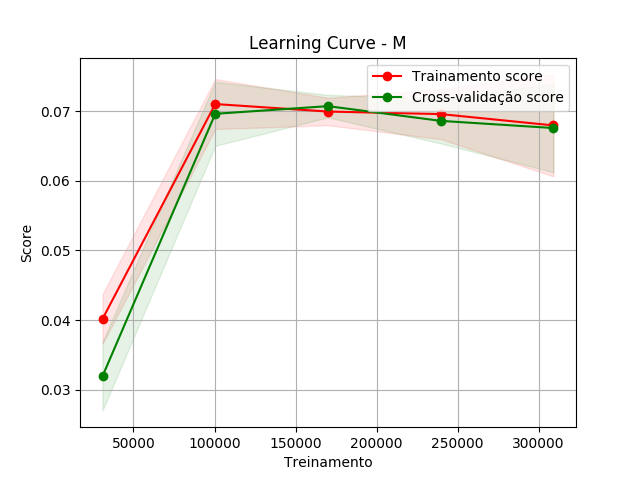
\includegraphics[scale=0.2]{../graphs/curveM.png}}
		}
	}
	\quad
	\subfloat[Curva de aprendizado para covariância do timbre.]{
		{
			\setlength{\fboxsep}{1pt}
			\setlength{\fboxrule}{1pt}
			\fbox{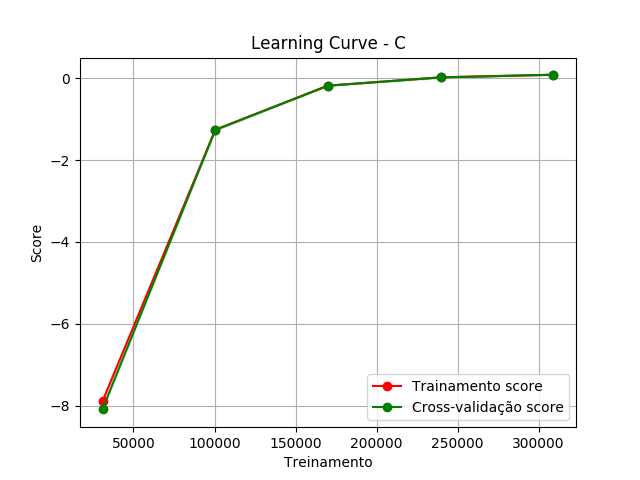
\includegraphics[scale=0.2]{../graphs/curveC.png}}
		}
	}
	\quad
	\subfloat[Curva de aprendizado para média e covariância do timbre.]{
		{
			\setlength{\fboxsep}{1pt}
			\setlength{\fboxrule}{1pt}
			\fbox{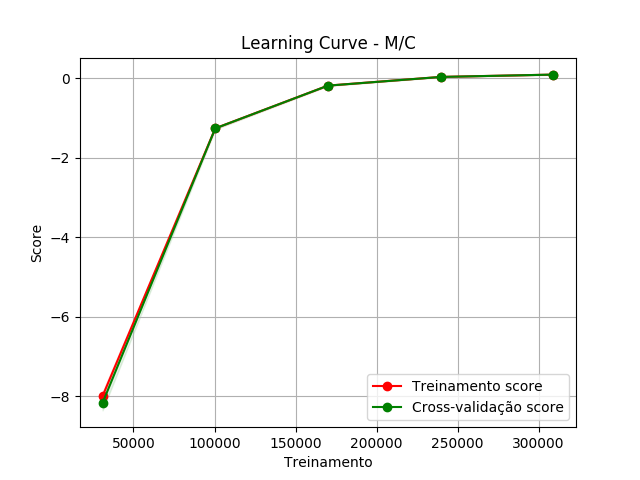
\includegraphics[scale=0.2]{../graphs/curveMC.png}}
		}
	}
	\quad
	\subfloat[Curva de aprendizado para média e covariância do timbre e normalização separada.]{
		{
			\setlength{\fboxsep}{1pt}
			\setlength{\fboxrule}{1pt}
			\fbox{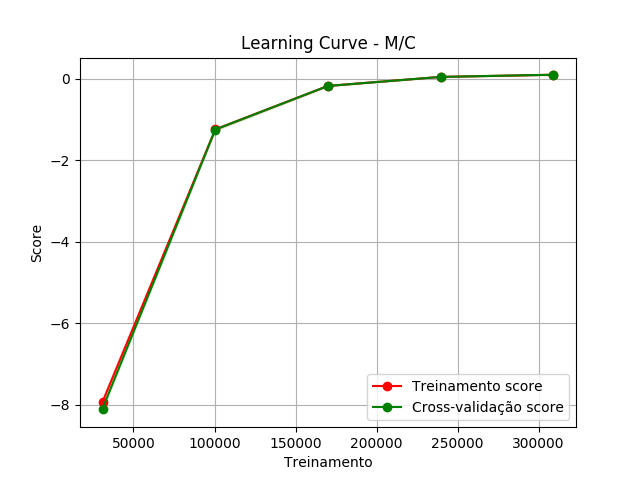
\includegraphics[scale=0.2]{../graphs/cuvreMC*.png}}
		}
	}
	\caption{Curvas de aprendizado para os diferentes modelos.}
	\label{fig:learningcurves}
\end{figure}


\subsection{Learning Rate}

O objetivo desta seção é mostrar como o \emph{learning rate} influência no resultado dos modelos, a Tabela \ref{tab:rates} mostra uma comparação dos resultados para diferentes \emph{learning rates} para as diversas combinações de features. Em todos os experimentos foram utilizados $100$ iterações.

\begin{table}[!h]
	\centering

	\begin{tabular}{ccccc} \\ \hline
		\textbf{Learning Rates} & \textbf{M/C*} & \textbf{M/C} & \textbf{C} & \textbf{M} \\ \hline
		\textbf{0,01}   & 7,71          & 7,60         & 7,49       & 7,87       \\
		\textbf{0,001}  & 7,33          & 7,42         & 7,53       & 7,77       \\
		\textbf{0,0001} & 7,34          & 7,54         & 7,57       & 7,80       \\ \hline
	\end{tabular}
	\caption{Comparação do resultado obtido com a métrica \textit{Mean Absolute Error} com diferentes \emph{learning rates}.}
	\label{tab:rates}
\end{table}

Pôde-se perceber que houve uma melhora nos resultados, a medida que se reduzia o \textit{learning rate}, isto é, o tamanho do \textit{learning rate} é inversamente proporcional a um melhor desempenho no treinamento do modelo. Os resultados mostrados para o \emph{learning rate} $= 0,0001$ são inferiores (e no caso, melhores) aos mostrados para os valores de $0,001$ nos modelos abordados. Contudo, para menores valores de tal parâmetro, o tempo de cômputo é maior, uma vez que demora sua convergência é demorada. Assim, para maiores valores do \textit{learning rate}, o método pode convergir mais rápido ou nunca atingir a solução esperada para tal problema.

Escolher o melhor modelo baseado no \textit{learning rate} pode ser uma tarefa difícil, pois há necessidade de considerar o tempo de processamento e as melhorias nos resultados. Neste trabalho, consideramos que o valor $0,001$ foi melhor, devido a baixa diferença entre os resultados e o número de iterações que foram utilizadas. A Figura \ref{fig:learningrate} mostra como o número de iterações afeta a descida do gradiente mostrando a função de custo (\emph{Mean Squared Error}).

\subsection{Modelos com equações polinomiais mais complexas}

Com intuito de testar modelos mais complexos, foi utilizado de equações polinomiais para representar os dados. Esse modelo se torna muito caro dependendo da quantidade de dados, devido a isso não foi possível fazer todos os testes.

A Tabela \ref{tab:comp} mostra os resultados obtidos pela equação polinomial de segundo grau, para a equação normal apenas as \emph{features} de média foram testadas, utilizando um maior número de \emph{features} o custo computacional fica muito elevado. Desta forma, como o intuito do trabalho é testar diversas estratégia, foi optado por não realizar esses experimentos. Todos os resultados foram obtidos utilizando \emph{learning rate} igual a $0,01$.

\begin{table}[!h]
	\centering

	\begin{tabular}{ccccc} \\ \hline
		\backslashbox{\textbf{Modelos}}{\textbf{Features}} & \textbf{M/C*} & \textbf{M/C} & \textbf{C} & \textbf{M} \\ \hline
		\textbf{Gradiente}      & 7,54     & 7,63         & 7,50       & 7,63  \\
		\textbf{Eq Normal}      & -       & -         & -       & 7,58    \\ \hline
	\end{tabular}
	\caption{Resultados da métrica \textit{Mean Absolute Error} usando diferentes características para as equações de segundo grau.}
	\label{tab:comp}
\end{table}

A tabela mostra que os resultados utilizando a equação polinomial de segundo grau foram um pouco melhores que a linear, esses resultados poderiam ser ainda mais melhorados utilizando mais iterações. Além deste experimento, foi feito um experimento utilizando de uma equação polinomial de terceiro grau.

Para esse modelo foi utilizado somente as \emph{features} que representam o médio do timbre, o motivo é que o alto número de dados tornava o modelo muito lento para generalizar. O resultado deste experimento foi de 7,58 \emph{Mean Absolute Error}, ou seja, uma pequena melhora foi obtida em relação a equação polinomial de segunda ordem.



\subsection{Resultados na base de testes }

Esta seção tem como objetivo verificar nossos modelos no base de testes, para todo o processo de treinamento foram utilizados dados normalizados. Além disso, para a descida de gradiente foi utilizado o \emph{learning rate} 0,001 que foi o que proporcionou o melhor resultado quando utilizando 100 iterações. A Tabela \ref{tab:result} mostra os resultados obtidos com as utilizando funções de primeiro grau, que e mostraram melhor no decorrer do trabalho.


\begin{table}[!h]
	\centering

	\begin{tabular}{ccccc}
		\hline
		& \textbf{M/C*} & \textbf{M/C} & \textbf{C} & \textbf{M} \\ \hline
		Gradiente & 7,22          & 7,34         & 7,66       & 7,76       \\
		Eq Normal & 7,23          & 7,31         & 7,46       & 7,82       \\ \hline
	\end{tabular}
	\caption{Resultados dos modelos lineares na base de teste.}
	\label{tab:result}
\end{table}

Pode-se perceber que os resultados foram similares com os encontrados durante a cross-validação, o que indica que nosso modelo pode aprender e predizer de forma a reduzir o erro esperado. Podemos concluir também que outras técnicas poderiam ter sido aplicadas para tornar possível os testes em modelos mais complexos que utilizassem de equações polinomiais.


\section{Conclusão} \label{sec:conc}

Regressão linear pode ser uma forma muito eficaz de predizer dados contínuos, a mesma se mostrou capaz de predizer os anos das música de forma a manter o erro médio absoluto baixo. O trabalho também proporcionou uma visão do quão importante a escolha das \emph{features} pode ser, assim como as vantagens da normalização dos dados.


\begin{thebibliography}{00}
%\bibitem{b1} Christopher M. Bishop. ``Pattern Recognition and Machine Learning''. Springer-Verlag New York, Inc., Secaucus, NJ, USA, 2006.
\bibitem{b1} Aurélien Géron ``Hands-On Machine Learning with Scikit-Learn and TensorFlow
Concepts, Tools, and Techniques to Build Intelligent Systems". O'Reilly Media, March 2017.
\end{thebibliography}


\end{document}
